%
% ritzAufProblem.tex 
%
% 
%
% !TEX root = ../../buch.tex
% !TEX encoding = UTF-8
%

\usetikzlibrary{pgfplots.fillbetween}

\section{Ritz-Verfahren für das Antennenproblem\label{antennen:ritzAnw}}

%todo CHAPTER REFERENZ
Wie in \ref{antennen:Geom} erwähnt, kann dank der Symmetrie das Problem nur auf eine Ecke abgebildet werden. 
Diese Ecke wird nun geschickt, wie in der Abbildung \ref{antennen:koordSysBsp} zu sehen, 
in ein Koordinatensystem gesetzt, welches erlaubt das Problem genauer zu analysieren.
%TODO bild ist weit weg  ILLEGAL
\begin{figure}
	\centering
	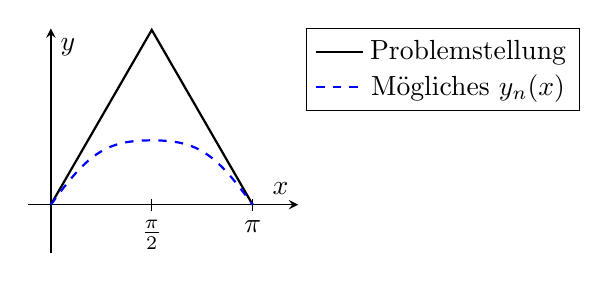
\begin{tikzpicture}
		\begin{axis}[
			scale=0.5,
			axis lines=middle,
			xlabel={$x$},
			ylabel={$y$},
			axis line style = {line width=0.5pt},
			tick style={line width=0.5pt, black},
			xtick={0, 1.5708, 3.14159},
			xticklabels={0, $\frac{\pi}{2}$, $\pi$},
			ytick=\empty,
			enlargelimits,
			clip=false,
			xmin=0, xmax=3.5,
			ymin=0, ymax=2,
			domain=0:pi, 
			samples=100,
			legend pos=outer north east,
			axis equal
			]
			% 3eck spitze
			\addplot[thick] coordinates {(0,0) (1.5708, pi*1.732/2) (3.14159, 0)};
			\addlegendentry{Problemstellung}
			
			\addplot[thick, blue, dashed, domain=0:3.14159, samples=100] {1.0882345*sin(deg(x))+0.0866761*sin(3*deg(x))};
			\addlegendentry{Mögliches $y_n(x)$}
		\end{axis}
	\end{tikzpicture}
	\caption{Problemstellung im Koordinatensystem.}
	\label{antennen:koordSysBsp}
\end{figure}

Um die Effizienz $\eta$ zu optimieren, soll mit der Approximationsfunktion
$y_n(x)$, wie in Kapitel \ref{antennen:Geom} erwähnt, die Fläche $A$ 
maximiert und die Länge $l$ minimiert werden.

\subsection{Ideale Approximationsfunktion\label{antennen:unsereApproxFunkt}}

Bei diesem Problem ist zu erwarten, dass die Lösung eine glatte und symmetrische
Funktion sein wird. Somit ergibt sich
\begin{equation}
	y_n(x)
	= 
	\sum_{k=1}^n a_k\sin((2k-1)x)
	\label{antennen:unserRitz}
\end{equation}
als ideale Approximationsfunktion. 

Diese Entwicklung wird auch Sinus-Fourier Reihe genannt
und wenn diese für $n=2$ ausgeschrieben wird, ergibt sich
\begin{equation}
	y_n(x)
	=
	a_1\sin(x)+a_2\sin(3x)
	\label{antennen:approxFunktn2}
\end{equation}
als Approximationsfunktion. Im weiteren Verlauf ist $y_n(x)$ \eqref{antennen:approxFunktn2} 
die endgültige Approximationsfunktion, mit der die Problemstellung angegangen wird.

\subsection{Nebenbedingungen von $y_n(x)$\label{antennen:nebenbedRitz}}

Eine Nebenbedingung ist es, dass bei $y_n(0)$ und $y_n(\pi)$ die Funktion null sein muss.
Diese Nebenbedingung ist sehr wichtig für die Stetigkeit der finalen Antennenform, die optimiert wird.

Die Sinus-Fourier Reihe \eqref{antennen:unserRitz} hat eine weitere gute Eigenschaft, 
die ersichtlich wird, wenn man das gleiche Koordinatensystem wie bei der Abbildung \ref{antennen:koordSysBsp}
benutzt und $y_n(x)$ mit beispielsweise den Koeffizienten $a_1=a_2=1$ plottet.

%TODO bild ist weit weg  ILLEGAL
\begin{figure}
	\centering
	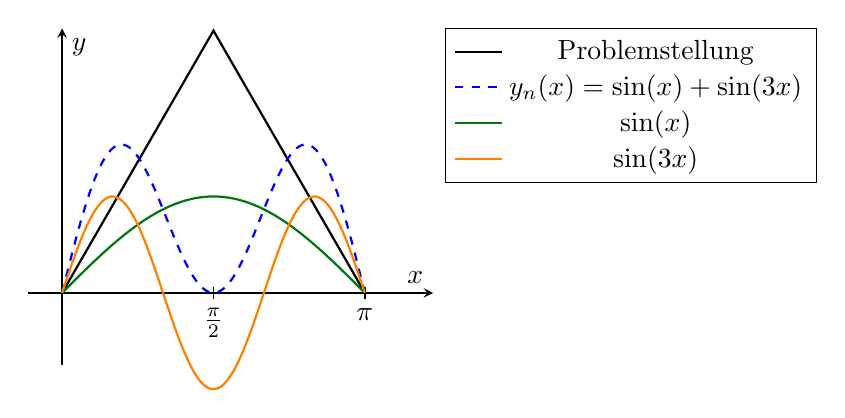
\begin{tikzpicture}
		\definecolor{clrGreen}{RGB}{0, 117, 18}
		\begin{axis}[
			scale=0.75,
			axis lines=middle,
			xlabel={$x$},
			ylabel={$y$},
			axis line style = {line width=0.5pt},
			tick style={line width=0.5pt, black},
			xtick={0, 1.5708, 3.14159},
			xticklabels={0, $\frac{\pi}{2}$, $\pi$},
			ytick=\empty,
			enlargelimits,
			clip=false,
			xmin=0, xmax=3.5,
			ymin=0, ymax=2,
			domain=0:pi, 
			samples=100,
			legend pos=outer north east,
			axis equal
			]
			% 3eck spitze
			\addplot[thick] coordinates {(0,0) (1.5708, pi*1.732/2) (3.14159, 0)};
			\addlegendentry{Problemstellung}
			
			\addplot[thick, blue, dashed, domain=0:3.14159, samples=100] {sin(deg(x))+sin(3*deg(x))};
			\addlegendentry{$y_n(x) = \sin(x)+\sin(3x)$}
			
			\addplot[thick, clrGreen, domain=0:3.14159, samples=100] {sin(deg(x))};
			\addlegendentry{$\sin(x)$}
			
			\addplot[thick, orange, domain=0:3.14159, samples=100] {sin(3*deg(x))};
			\addlegendentry{$\sin(3x)$}
		\end{axis}
	\end{tikzpicture}
	\caption{Nebenbedingungen im Koordinatensystem.}
	\label{antennen:nebenbedGrafik}
\end{figure}

In der Abbildung \ref{antennen:nebenbedGrafik} ist zu sehen, dass dank der Punktsymmetrie 
der ungeraden Sinus-Funktionen, die Nebenbedingungen
\begin{equation}
	\begin{aligned}
		y_n(0)
		&=
		0
		\\
		y_n(\pi)
		&=
		0
	\end{aligned}
\label{antennen:nebenbed3eck}
\end{equation}
\em immer erfüllt \em sind. Im weiteren Verlauf werden diese 
Nebenbedingungen somit nicht mehr beachtet.

\subsection{Die zu optimierende Funktion \label{antennen:optmFunktion}}

%Die beste Fläche ist auch gerade die beste Fläche im quadrat \qed

Abstrahieren wir das Problem nun ein bisschen. Anstelle der Fläche $A$ reden wir nun von 
der Funktion $f$ und aus der Länge $l$ wird die Nebenbedingung $n$. 

An dieser Stelle sind unsere Koeffizienten $a_k$ konkret zu bestimmen. 
Somit sind die neu erwähnten Funktionen 

\begin{equation}
\begin{aligned}
	A
	\rightarrow
	f(a_1,\ldots,a_k)
	\rightarrow
	f(a_1,a_2)
	&=
	\int\limits_{0}^{\pi} y_n(x,a_1,a_2)\, dx
	\\
	l
	\rightarrow
	n(a_1,\ldots,a_k)
	\rightarrow
	n(a_1,a_2)
	&=
	\int\limits_{0}^{\pi} \sqrt{1+y_n'(x, a_1, a_2)^2}\, dx
\end{aligned}
\label{antennen:lagrangeNamen}
\end{equation}
auch in deren Abhängigkeit in \eqref{antennen:lagrangeNamen} zu sehen. Wie schon erwähnt, 
ist das Problem hier auf zwei Koeffizienten beschränkt. 

Die Fläche unter der Kurve ergibt sich aus dem Integral der Funktion, 
währenddessen man für die Länge, also den oberen Rand der Funktion, 
zusätzlich die erste Ableitung auch noch braucht

Die Nebenbedingung $n$ setzen wir nun gleich einer konstanten Länge
\begin{equation}
n(a_1, a_2)
=
l
\label{antennen:constNebenbed}
\end{equation}
und wie jede gute Nebenbedingung setzen wir diese noch gleich null:

\begin{equation}
\begin{aligned}
	n(a_1, a_2) - l
	&=
	0
	\\
	n(a_1, a_2, l)
	&=
	0.
\label{antennen:fertigeNebenbed}
\end{aligned}
\end{equation}
Nun kann die zu optimierende Funktion

\begin{equation}
F(x,a_1,a_2,\lambda)
= 
f(a_1,a_2)+\lambda \: n(a_1,a_2, l)
\end{equation}
definiert werden. Dazu wird die Funktion $f$ mit der Nebenbedingung $n(a_1,a_2,l)$ und einem
Multiplikator $\lambda$ addiert.

\subsection{Das endlichdimensionale Gleichungssystem\label{antennen:lagrangeGLsys}}

Die Funktion $F$ möchte man nun ableiten und gleich 0 setzen. Das heisst in diesem Kontext
den Gradienten

\begin{equation}
	\nabla F 
	=
	\begin{pmatrix} 
		\frac{\displaystyle\strut\partial F}{\displaystyle\strut\partial a_1} 
		\\ 
		\frac{\displaystyle\strut\partial F}{\displaystyle\strut\partial a_2}  
	\end{pmatrix} 
	= 
	\vec{0} \Rightarrow
	\left\{
	\begin{aligned}
		\frac{\partial F}{\partial a_1} = 0 \\
		\frac{\partial F}{\partial a_2} = 0
	\end{aligned}
	\right.
	\label{antennen:lagrangeGrad}
\end{equation}
berechnen und dem Nullvektor gleichsetzen. Dabei entsteht hier ein 
$n+1$ dimensionales Gleichungssystem aus \eqref{antennen:lagrangeGrad} und \eqref{antennen:fertigeNebenbed},
wobei $n$ die Anzahl der Koeffizienten ist.

An dieser Stelle wird ersichtlich, was diese Kapitel von den anderen unterschiedet. Mit dem Verfahren nach Ritz  
kann ein unendlichdimensionales
Problem wie z. B. in Kapitel \ref{buch:chapter:nebenbedingungen}, in ein endlich dimensionales verwandelt werden. 
Konkret bedeutet dies, dass wir keine Differentialgleichung lösen müssen, sondern, 
das nichtlineare Gleichungssystem, welches wir zuvor erhalten haben.

Das Gleichungssystem, in diesem Fall mit 
2 Koeffizienten, kann nun als
\begin{equation}
	\begin{aligned}
		\int_0^\pi \sin (x) dx
		&=
		-\lambda \int_0^\pi \frac{\left(a_1 \cos (x)+3 a_2 \cos (3 x)\right) 
			\cos (x)}{\sqrt{\left(a_1 \cos (x)+3 a_2 \cos (3 x)\right)^2+1}} \, dx \\
		\int_0^\pi \sin (3 x) dx
		&=
		-\lambda \int_0^\pi \frac{3\left(a_1 \cos (x)+3 a_2 \cos (3 x)\right) 
			\cos (3 x)}{\sqrt{\left(a_1 \cos (x)+3 a_2 \cos (3 x)\right)^2+1}} \, dx \\
		l
		&=
		\int_0^\pi \sqrt{\left(a_1 \cos (x)+3 a_2 \cos (3 x)\right)^2+1} \, dx
	\end{aligned}
	\label{antennen:lagrangeGradKonkret}
\end{equation}
ausgeschrieben werden. 

\subsection{Das Gleichungssystem lösen\label{antennen:glSysSolve}}

Ein gutes Verfahren, welches sich zur Lösung des Gleichungssystems 
\eqref{antennen:lagrangeGradKonkret} anbietet, ist das Gradientenverfahren. Dieses 
iterative Verfahren eignet sich hervorragend zur Minimierung 
einer Funktion, indem schrittweise in Richtung des steilsten Abstiegs,
also des Gradienten aus der Gleichung \eqref{antennen:lagrangeGrad},
fortgeschritten wird. 

\begin{figure}
	\centering
	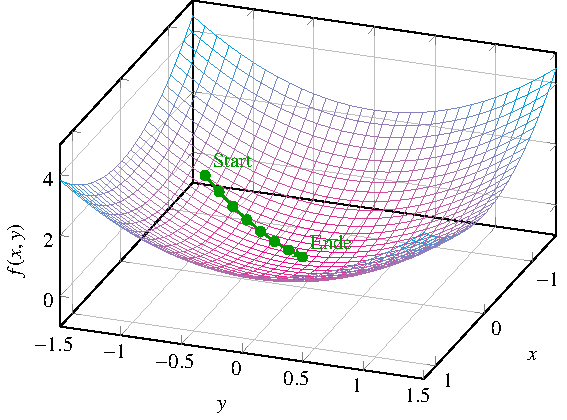
\includegraphics{papers/antennen/images/gradienteverfahren.pdf}
	\caption{Gradientenverfahren auf $f(x,y)=x^2+y^2$.}
	\label{antennen:gradverfahrenBSP}
\end{figure}

Ein Beispiel dafür wie das Verfahren aussehen kann, wird in 
Abbildung \ref{antennen:gradverfahrenBSP} gezeigt. Man nimmt irgendeinen Startpunkt
und geht Schritt für Schritt in Richtung des negativen Gradienten $-\nabla f$.
Mit der Funktion $f(x,y)=x^2+y^2$ ist dieses Verfahren recht einfach zu 
implementieren und auszuführen.

Dieses Verfahren kommt jedoch auch mit einigen Tücken. Bei komplexen Funktionen muss die 
Schrittgrösse und Toleranz geschickt gewählt werden, da sonst die Gefahr gross ist,
bei \em lokalen \em Minima stecken zu bleiben, obwohl ein \em globales \em Minimum gesucht ist.

Da wir in unserer Arbeit ohnehin die Python-Bibliothek \texttt{SymPy} verwendet haben, 
um symbolische Berechnungen durchzuführen und automatisch $n$ Koeffizienten zu berechnen, 
konnten wir das Gleichungssystem \eqref{antennen:lagrangeGradKonkret} mithilfe der Funktion 
\texttt{nsolve()} lösen.
Den Code findet der Leser unter \cite{antennen:codeKoeff}.

\subsection{Die Lösung verstehen\label{antennen:auswertung}}

Die Abbildung \ref{antennen:plotskoeff} zeigt, wie sich die Lösung visuell mit mehr 
Koeffizienten verändert. Auf der x-Achse sieht man jeweils eine beliebige Distanz von \emph{$\pi$}.
Diese Distanz verbindet die Funktion $y_n(x)$ mit einer
fixen Länge $l$. Wie lang die verschiedenen Längen genau sind, ist hierbei noch irrelevant.

Das Ergebnis ist die \emph{optimale Form} mit
maximaler Fläche unter der Funktion. Mit mehr Koeffizienten $n$ kann die Funktion
immer mehr Fläche aufspannen. Eine sehr interessante Länge jedoch sollte man
genauer unter die Lupe nehmen. 

Zuvor wurde in Kapitel \ref{buch:chapter:nebenbedingungen} das Problem von Dido
behandelt, bei dem es auch darum ging, die Fläche zu \emph{maximieren} und den Umfang oder die Länge $l$ zu 
\emph{minimieren}. 
Dort kam eine Form mit konstanter zweiter Ableitung, also anders ausgedrückt
der Kreis, als Lösung hervor. Somit ist die für uns interessante Länge $l$ der Durchmesser eines Kreises. Dieser wichtige Vergleich wird in \ref{antennen:vergleich} gemacht und genauer erläutert.

% TODO nicht gute position,  illegal
\begin{figure}
	\centering
	
	\definecolor{color1}{rgb}{1.0, 0.0, 1.0}
	\definecolor{color2}{rgb}{0.75, 0.0, 1.0}
	\definecolor{color3}{rgb}{0.5, 0.0, 1.0}
	\definecolor{color4}{rgb}{0.25, 0.0, 1.0}
	
	% 2 koeff
	\begin{subfigure}
		\centering
		\begin{tikzpicture}
			\begin{axis}[
				title={$n=2$ Koeffizienten},
				domain=0:pi,
				samples=100,
				ymin=0, ymax=3.5,
				xmin=0, xmax=3.5,
				axis lines=middle,
				xlabel={$x$},
				ylabel={$y$},
				axis line style = {line width=0.5pt},
				tick style={line width=0.5pt, black},
				xtick={0, 1.5708, 3.14159},
				xticklabels={0, $\frac{\pi}{2}$, $\pi$},
				ytick={0, 1, 2, 3},
				width=6cm, height=4cm
				]
				\addplot[thick, color1] {1.08823455130519*sin(deg(x)) + 0.0866761835928106*sin(3*deg(x))};
				\addplot[thick, color2] {1.81055138481242*sin(deg(x)) + 0.195685048731416*sin(3*deg(x))};
				\addplot[thick, color3] {2.46066609594305*sin(deg(x)) + 0.301243389027199*sin(3*deg(x))};
				\addplot[thick, color4] {3.08456094286871*sin(deg(x)) + 0.402479943701422*sin(3*deg(x))};
			\end{axis}
		\end{tikzpicture}
	\end{subfigure}%
	\hfill
	% 3 koeff
	\begin{subfigure}
		\centering
		\begin{tikzpicture}
			\begin{axis}[
				title={$n=3$ Koeffizienten},
				domain=0:pi,
				samples=100,
				ymin=0, ymax=3.5,
				xmin=0, xmax=3.5,
				axis lines=middle,
				xlabel={$x$},
				ylabel={$y$},
				axis line style = {line width=0.5pt},
				tick style={line width=0.5pt, black},
				xtick={0, 1.5708, 3.14159},
				xticklabels={0, $\frac{\pi}{2}$, $\pi$},
				ytick={0, 1, 2, 3},
				width=6cm, height=4cm
				]
				\addplot[thick, color1] {1.14063451060611*sin(deg(x)) + 0.108169939153489*sin(3*deg(x)) + 0.0268323654703764*sin(5*deg(x))};
				\addplot[thick, color2] {1.85437292911293*sin(deg(x)) + 0.253791821832382*sin(3*deg(x)) + 0.0683318364481152*sin(5*deg(x))};
				\addplot[thick, color3] {2.50955540772763*sin(deg(x)) + 0.402071210261300*sin(3*deg(x)) + 0.110183839692472*sin(5*deg(x))};
				\addplot[thick, color4] {3.14502916280716*sin(deg(x)) + 0.548044536721918*sin(3*deg(x)) + 0.150139877796318*sin(5*deg(x))};
			\end{axis}
		\end{tikzpicture}
	\end{subfigure}
	
	\vspace{0.5cm} 
	
	% 4l koeff
	\begin{subfigure}
		\centering
		\begin{tikzpicture}
			\begin{axis}[
				title={$n=4$ Koeffizienten},
				domain=0:pi,
				samples=100,
				ymin=0, ymax=3.5,
				xmin=0, xmax=3.5,
				axis lines=middle,
				xlabel={$x$},
				ylabel={$y$},
				axis line style = {line width=0.5pt},
				tick style={line width=0.5pt, black},
				xtick={0, 1.5708, 3.14159},
				xticklabels={0, $\frac{\pi}{2}$, $\pi$},
				ytick={0, 1, 2, 3},
				width=6cm, height=4cm
				]
				\addplot[thick, color1] {1.08336686654360*sin(deg(x)) + 0.102013525169225*sin(3*deg(x)) + 0.0292728737553532*sin(5*deg(x)) + 0.0100642932737197*sin(7*deg(x))};
				\addplot[thick, color2] {1.80275228117654*sin(deg(x)) + 0.262223597024550*sin(3*deg(x)) + 0.0898544624243682*sin(5*deg(x)) + 0.0312039886658123*sin(7*deg(x))};
				\addplot[thick, color3] {2.46107632379109*sin(deg(x)) + 0.430953350464770*sin(3*deg(x)) + 0.156100515783400*sin(5*deg(x)) + 0.0535838810399717*sin(7*deg(x))};
				\addplot[thick, color4] {3.10156229609598*sin(deg(x)) + 0.599148439503026*sin(3*deg(x)) + 0.221465165912620*sin(5*deg(x)) + 0.0748051312645227*sin(7*deg(x))};
			\end{axis}
		\end{tikzpicture}
	\end{subfigure}%
	\hfill
	% 5 koeff
	\begin{subfigure}
		\centering
		\begin{tikzpicture}
			\begin{axis}[
				title={$n=5$ Koeffizienten},
				domain=0:pi,
				samples=100,
				ymin=0, ymax=3.5,
				xmin=0, xmax=3.5,
				axis lines=middle,
				xlabel={$x$},
				ylabel={$y$},
				axis line style = {line width=0.5pt},
				tick style={line width=0.5pt, black},
				xtick={0, 1.5708, 3.14159},
				xticklabels={0, $\frac{\pi}{2}$, $\pi$},
				ytick={0, 1, 2, 3},
				width=6cm, height=4cm
				]
				\addplot[thick, color1] {1.08242048596654*sin(deg(x)) + 0.103364847431102*sin(3*deg(x)) + 0.0311161489593337*sin(5*deg(x)) + 0.0125977513219976*sin(7*deg(x)) + 0.00512952717128434*sin(9*deg(x))};
				\addplot[thick, color2] {1.79915900016821*sin(deg(x)) + 0.271669937694202*sin(3*deg(x)) + 0.102270415943148*sin(5*deg(x)) + 0.0453106859569591*sin(7*deg(x)) + 0.0178553921145572*sin(9*deg(x))};
				\addplot[thick, color3] {2.45687381390258*sin(deg(x)) + 0.451721838817908*sin(3*deg(x)) + 0.183206206667679*sin(5*deg(x)) + 0.0827190790444953*sin(7*deg(x)) + 0.0317715747685065*sin(9*deg(x))};
				\addplot[thick, color4] {3.09881979748560*sin(deg(x)) + 0.632286666812462*sin(3*deg(x)) + 0.264348386834190*sin(5*deg(x)) + 0.119443731427762*sin(7*deg(x)) + 0.0448574142367621*sin(9*deg(x))};
			\end{axis}
		\end{tikzpicture}
	\end{subfigure}
	
	\caption{Verschiedene Längen $l$ für $y_n(x)$ mit verschieden vielen Koeffizienten.}
	\label{antennen:plotskoeff}
\end{figure}

\subsection{Vergleich mit der exakten Lösung\label{antennen:vergleich}}

Die Abbildung \ref{antennen:vergleichKreis} vergleicht unsere Lösung\footnotemark{}, also die 
Funktion $y_n(x)$ optimiert für den halben Kreisumfang eines Kreises mit Durchmesser $\pi$. 
Einfacher ausgedrückt $l=\frac{\pi^2}{2}$.

\footnotetext{Das ausrechnen der acht Koeffizienten mit dem Python-Skript \cite{antennen:codeKoeff}
dauerte je nach Maschine und Anfangswerte, 5 bis 10 Minuten.}

Man sieht hier schon recht gut, dass $y_n(x)$ der
exakten Lösung, dem Kreis, konvergiert. Dies ist
natürlich kein wasserfester Beweis, hier aber völlig  
ausreichend. 

\begin{figure}
	\centering
	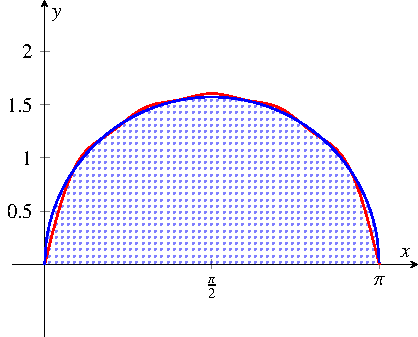
\includegraphics{papers/antennen/images/koeffVergleichKreis.pdf}
	\caption{$y_n(x)$ mit 8 Koeffizienten verglichen mit einem Kreis mit Durchmesser $\pi$.}
	\label{antennen:vergleichKreis}
\end{figure}














